\section{O Programa} \label{sec:programa}

% TODO: testar 3.6+

A ferramenta foi desenvolvida e testada para as versões de Python \autocite{python} 3.6 ou superior. Também foram utilizados os pacotes OpenCV \autocite{opencv}, para entrada e saída de imagens, Numpy \autocite{numpy}, para operações vetorizadas com a imagem, e Matplotlib \autocite{matplotlib}, para opções de cores de fundo.

\subsection{Código-Fonte}

    Neste trabalho foi elaborada a ferramenta \texttt{transforma.py} que faz a transformação da imagem e aplicação da interpolação. O código responsável pelas operações podem ser encontrados na pasta \texttt{lib}, como apresentado a seguir.

    \begin{description}[leftmargin=1.5em]

        \item[transforma.py] Ferramenta de transformação da imagem.

        \item[lib] Conjunto de arquivos com implementações para cada funcionalidade da ferramenta.

        \begin{description}

            \item[idx.py] Criação, transformação e acesso com as coordenadas de cada pixel da imagem.

            \item[linop.py] Operações lineares puras de escalonamento, rotação e translação.

            \item[opimg.py] Operações lineares mais aplicadas a imagem, sempre ajustando o resultado para a origem e retornando os novos limites da imagem.

            \item[interp.py] Recuperação da imagem transformada por interpolação dos pontos.

            \item[args.py] Processamento dos argumentos da linha de comando.

            \item[inout.py] Tratamento de entrada e saída de imagens do programa.

            \item[tipos.py] Tipos para checagem estática \autocite{mypy} \autocite{pep484}.
        \end{description}
    \end{description}

    Todas as imagens base para o processamento discutido ao longo do texto estão presente na pasta \texttt{imagens}. Também existe o \textit{script} \texttt{run.sh} em Bash que refaz todos resultados apresentados neste relatório.

\subsection{Argumentos}

    A execução de ambos os programas deverá ser feita através do interpretador de Python 3.6+. Os exemplos de execuções neste relatório podem não funcionar nessa versão, devido à ordem com que os argumentos são interpretados \autocite{intermixed}. No entanto, o \textit{script} \texttt{run.sh} funciona em todas variantes especificadas.

    Todas as opções à seguir são apresentadas no texto de ajuda da ferramenta, que pode ser acessado com a \textit{flag} \mintinline{bash}{--help} ou apenas \mintinline{bash}{-h}. É possível habilitar a amostragem do tempo de execução, com a opção \mintinline{bash}{-v} ou \mintinline{bash}{--verboso}. Quando repetida, essa opção apresenta ainda mais detalhes da execução da ferramenta.

\subsubsection{Entrada e Saída}

    O único argumento obrigatório é o caminho da imagem de entrada, preferencialmente PNG, que deverá ser transformada. A imagem de saída é, por padrão, exibida em uma nova janela gráfica, mas pode ser salva em um arquivo com a opção \mintinline{bash}{--output SAIDA} ou \mintinline{bash}{-o SAIDA}.

    Se nenhum outro argumento for especificado, a ferramenta apenas clona a imagem de entrada. Por exemplo, a invocação a seguir gera uma imagem \texttt{saida.png} idêntica à entrada \texttt{imagens/baboon.png}.

    \begin{minted}{bash}
        $ python3 transforma.py imagens/baboon.png -o saida.png
    \end{minted}

\subsubsection{Transformações}

    \begin{wrapfigure}{L}{0.25\textwidth}
        \centering
        \includegraphics[width=0.2\textwidth]{exemplo.png}
        \caption{Exemplo de execução.}
        \label{fig:exemplo}
    \end{wrapfigure}

    A primeira transformação que pode ser feita na imagem é uma rotação no plano XY por um ângulo $\alpha$. Isso pode ser realizado com \mintinline{bash}{--angulo ALFA} ou \mintinline{bash}{-a ALFA}. Também pode ser feita uma rotação em torno do eixo Y, que é projetada em perspectiva para o plano original da imagem. A \textit{flag} para isso é \mintinline{bash}{--beta BETA} ou \mintinline{bash}{-b BETA}. Ambas opções tratam apenas de ângulos em graus. Os detalhes dessas transformações pode ser encontrado na \cref{sec:transformacoes}.


    Também temos as opções de escalonamento da imagem. A opção \mintinline{bash}{--escala ESCALA} ou \mintinline{bash}{-e ESCALA} recebe um fator de escala positivo e redimensiona cada pixel por esse fator, nas duas dimensões da imagem. Também pode ser especificada as dimensões da imagem resultante, com a \textit{flag} \mintinline{bash}{--dim ALTURA LARGURA} ou \mintinline{bash}{-d ALTURA LARGURA}. Apenas uma das opções de escala pode ser usada a cada invocação.

    As transformações são aplicadas na ordem com que aparecem nessa seção, ou seja, primeiro é feito a rotação no plano XY, depois a rotação em torno de Y com a projeção perspectiva, e por fim o redimensionamento. As entradas númericas também podem ser passadas por expressões matemáticas simples e podem usar funções da bibliotecas \mintinline{python}{math}. O exemplo abaixo usa algumas expressões para gerar a \cref{fig:exemplo}.

    \begin{minted}[style=vs]{bash}
        $ python3 transforma.py imagens/city.png -o saida.png \
            -a asin\(0.25\) -b deg\(pi/4\) -e 1/3
    \end{minted}

\subsubsection{Método de Interpolação}

    A ferramenta é capaz de interpolar de quatro métodos diferentes, escolhidos com a opção \mintinline{bash}{--metodo METODO} ou \mintinline{bash}{-m METODO}. Os métodos são: \mintinline{bash}{-m vizinho} (\cref{sec:interp:vizinho}), para interpolação pelo vizinho mais próximo, \mintinline{bash}{-m bilinear} (\ref{sec:interp:bilinear}), \mintinline{bash}{-m bicubica} (\ref{sec:interp:bicubica}) e \mintinline{bash}{-m lagrange} (\ref{sec:interp:lagrange}), que usa polinômios de Langrange. O padrão é \texttt{bilinear}.

\subsubsection{Cor do Fundo}

    \begin{wrapfigure}{L}{0.25\textwidth}
        \centering
        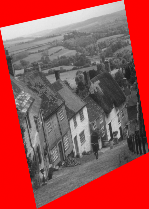
\includegraphics[width=0.2\textwidth]{exemplo2.png}
        \caption{Exemplo de execução.}
        \label{fig:exemplo2}
    \end{wrapfigure}

    Todas as transformações são feitas de forma que a imagem resultante seja uma caixa delimitadora da imagem transformada. No entanto, as rotações podem fazer com que a imagem transformada não seja retangular, o que deixa buracos na imagem resultante. Nesses casos, é aplicada uma cor de fundo em RGBA, representando a falta de informação.

    Por padrão, a cor de fundo é transparente, mas isso pode ser alterado com a \textit{flag} \mintinline{bash}{--cor COR} ou \mintinline{bash}{-c COR}. As opções de cores são tratadas pela função \mintinline{python}{to_rgba} \autocite{torbga}, então todas as cores da biblioteca Matplotlib são reconhecidas pela ferramenta. Uma opção extra \mintinline{python}{'transparente'} ou \mintinline{python}{'t'} é utilizada para representar o fundo transparente, usado como padrão.

    O exemplo a seguir gera uma imagem \cref{fig:exemplo2}, que é similar à \ref{fig:exemplo}, mas com fundo vermelho e construída por interpolação bicúbica.

    \begin{minted}[style=vs]{bash}
        $ python3 transforma.py imagens/city.png -o saida.png \
            -a asin\(0.25\) -b deg\(pi/4\) -e 1/3 -m bicubica -c red
    \end{minted}
